% !TEX TS-program = pdflatex
\documentclass[11pt, oneside]{article}
\usepackage[margin=1in]{geometry}                		
\geometry{letterpaper}            
\usepackage{graphicx}
\usepackage{mwe}
\usepackage{subcaption}

\usepackage{amssymb}

\title{Homework 2}
\author{Yiqi Tang}
%\date{}

\begin{document}
\maketitle

\vspace*{3ex}
\noindent
In HW2, we created several figures, first to examine error as a function of significant digits in estimating $\pi$, then, to look at the objective functions aParab13\_2, aParab13\_8, and wildN, and the errors associated with finding their respective global minimums. The figures below show the results. 


   \begin{figure}
     \centering
     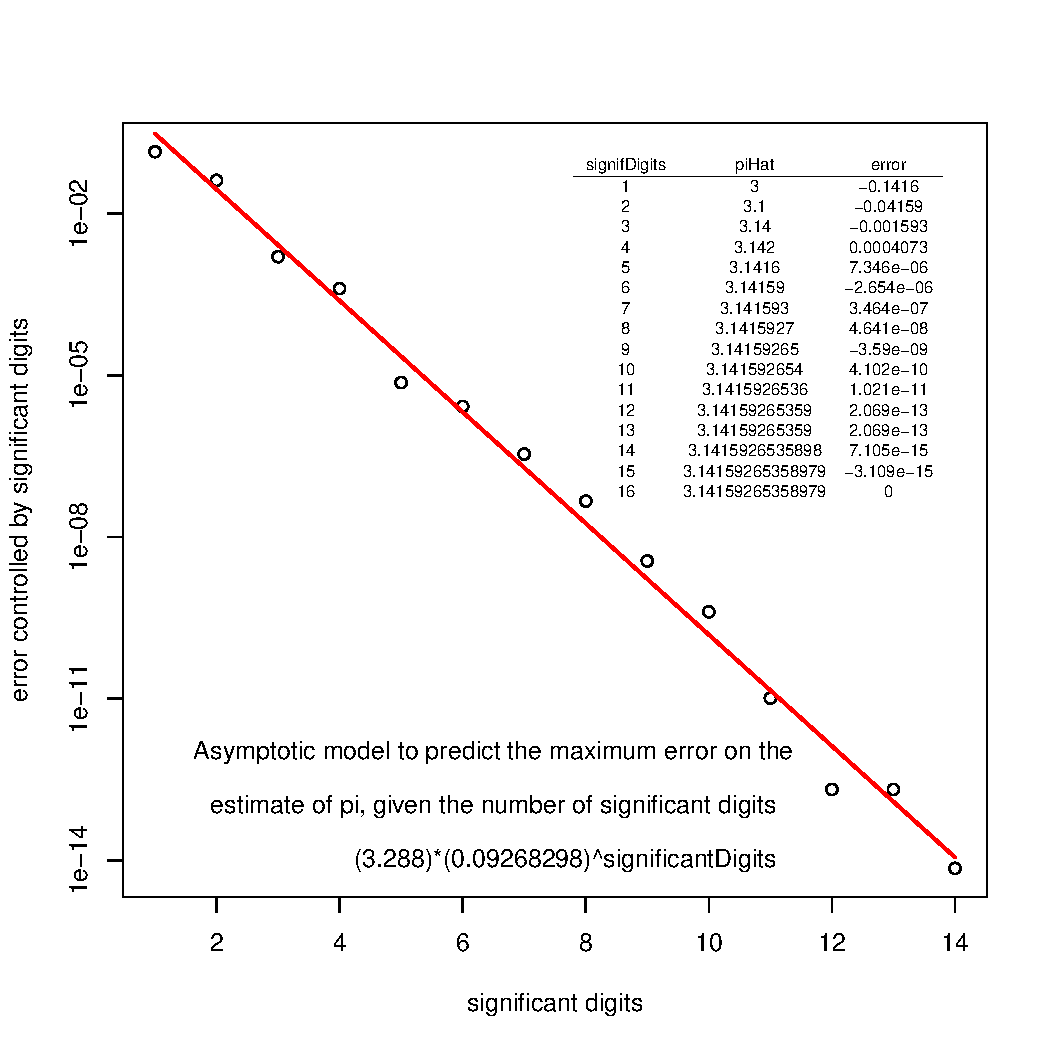
\includegraphics[width=1\linewidth]{fg_asym_pi_digits.pdf}
    \caption{Error as a Function of Significant Digits When Estimating the True Value of Pi}
   \end{figure}
   
   \begin{figure}
     \centering
     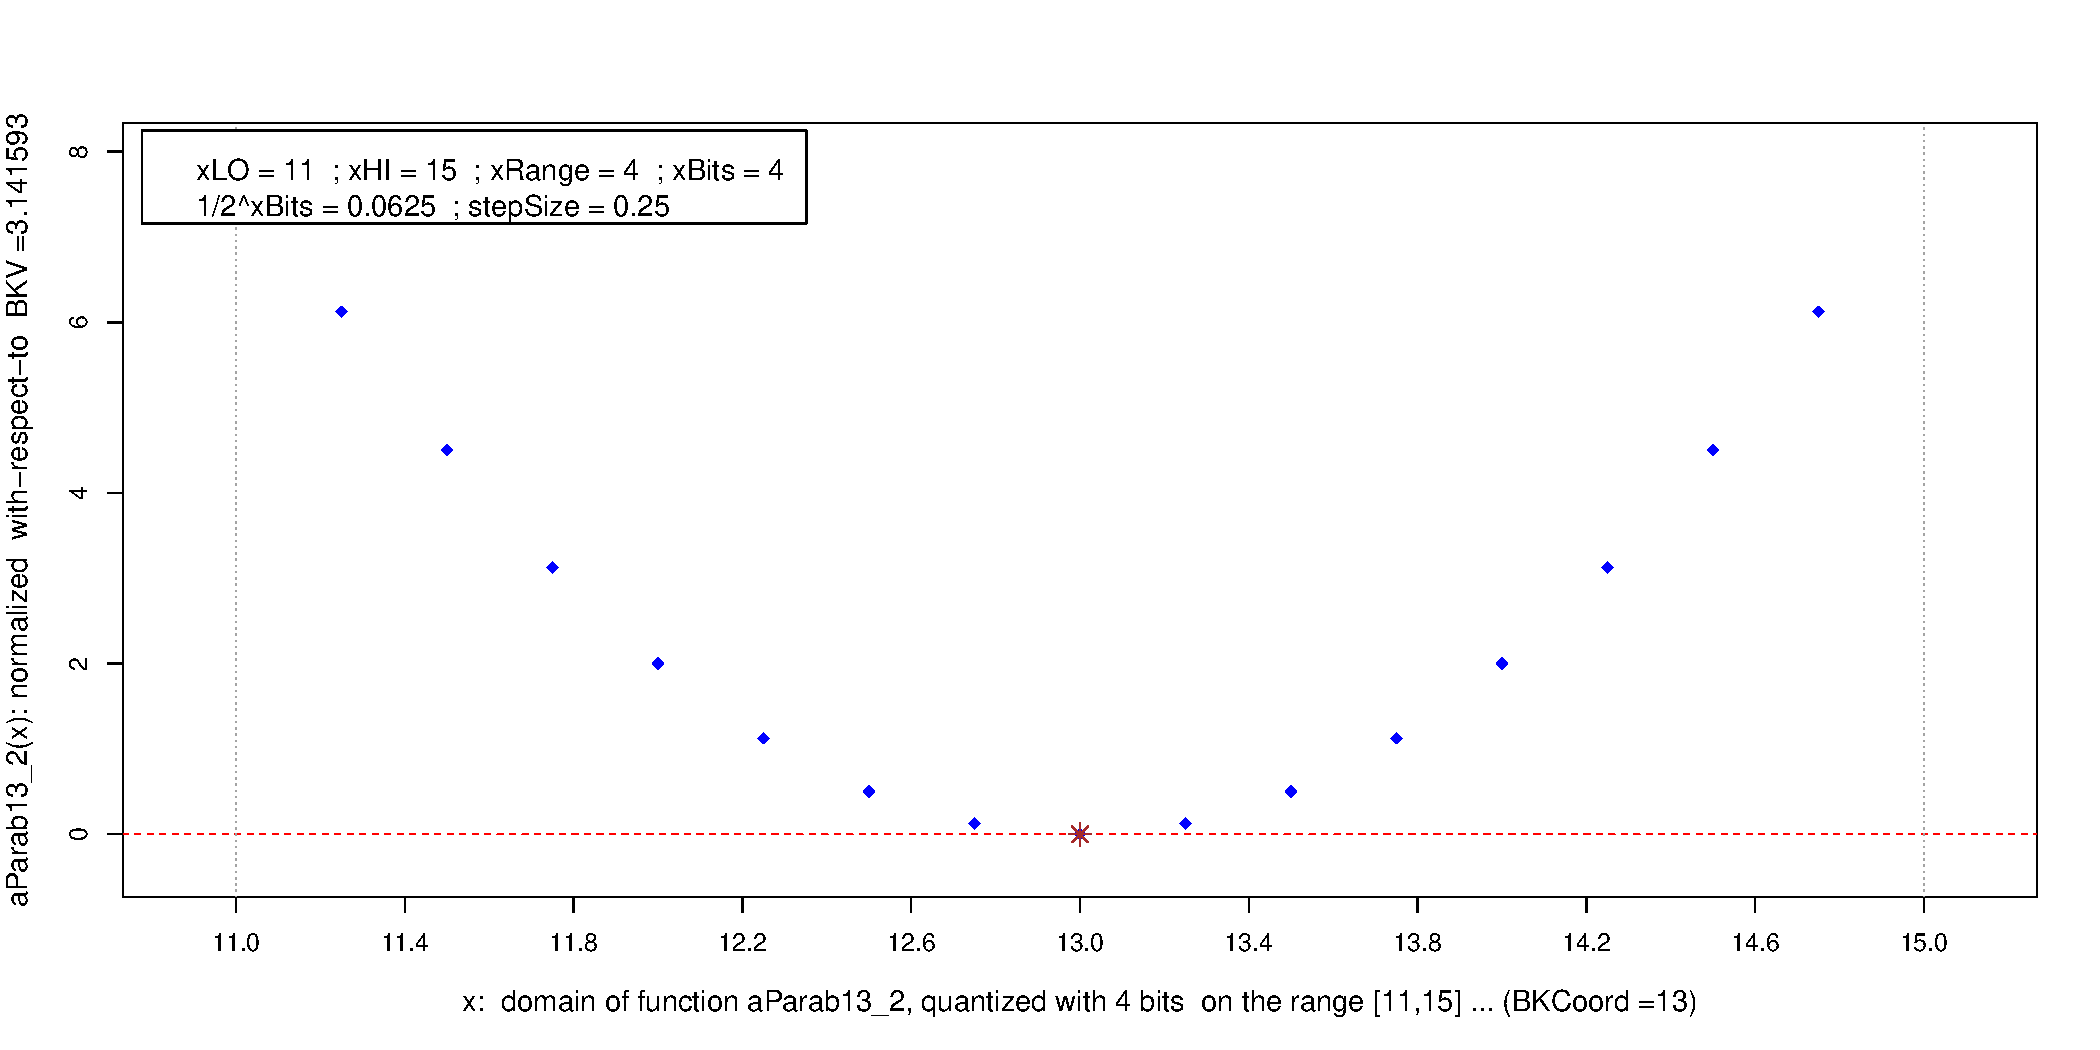
\includegraphics[width=1\linewidth]{fg_OF_aParab13_2_quant_exh.pdf}
    \caption{Function aParab13\_2 Normalized With Respect To BKV}
   \end{figure}
   
   \begin{figure}
     \centering
     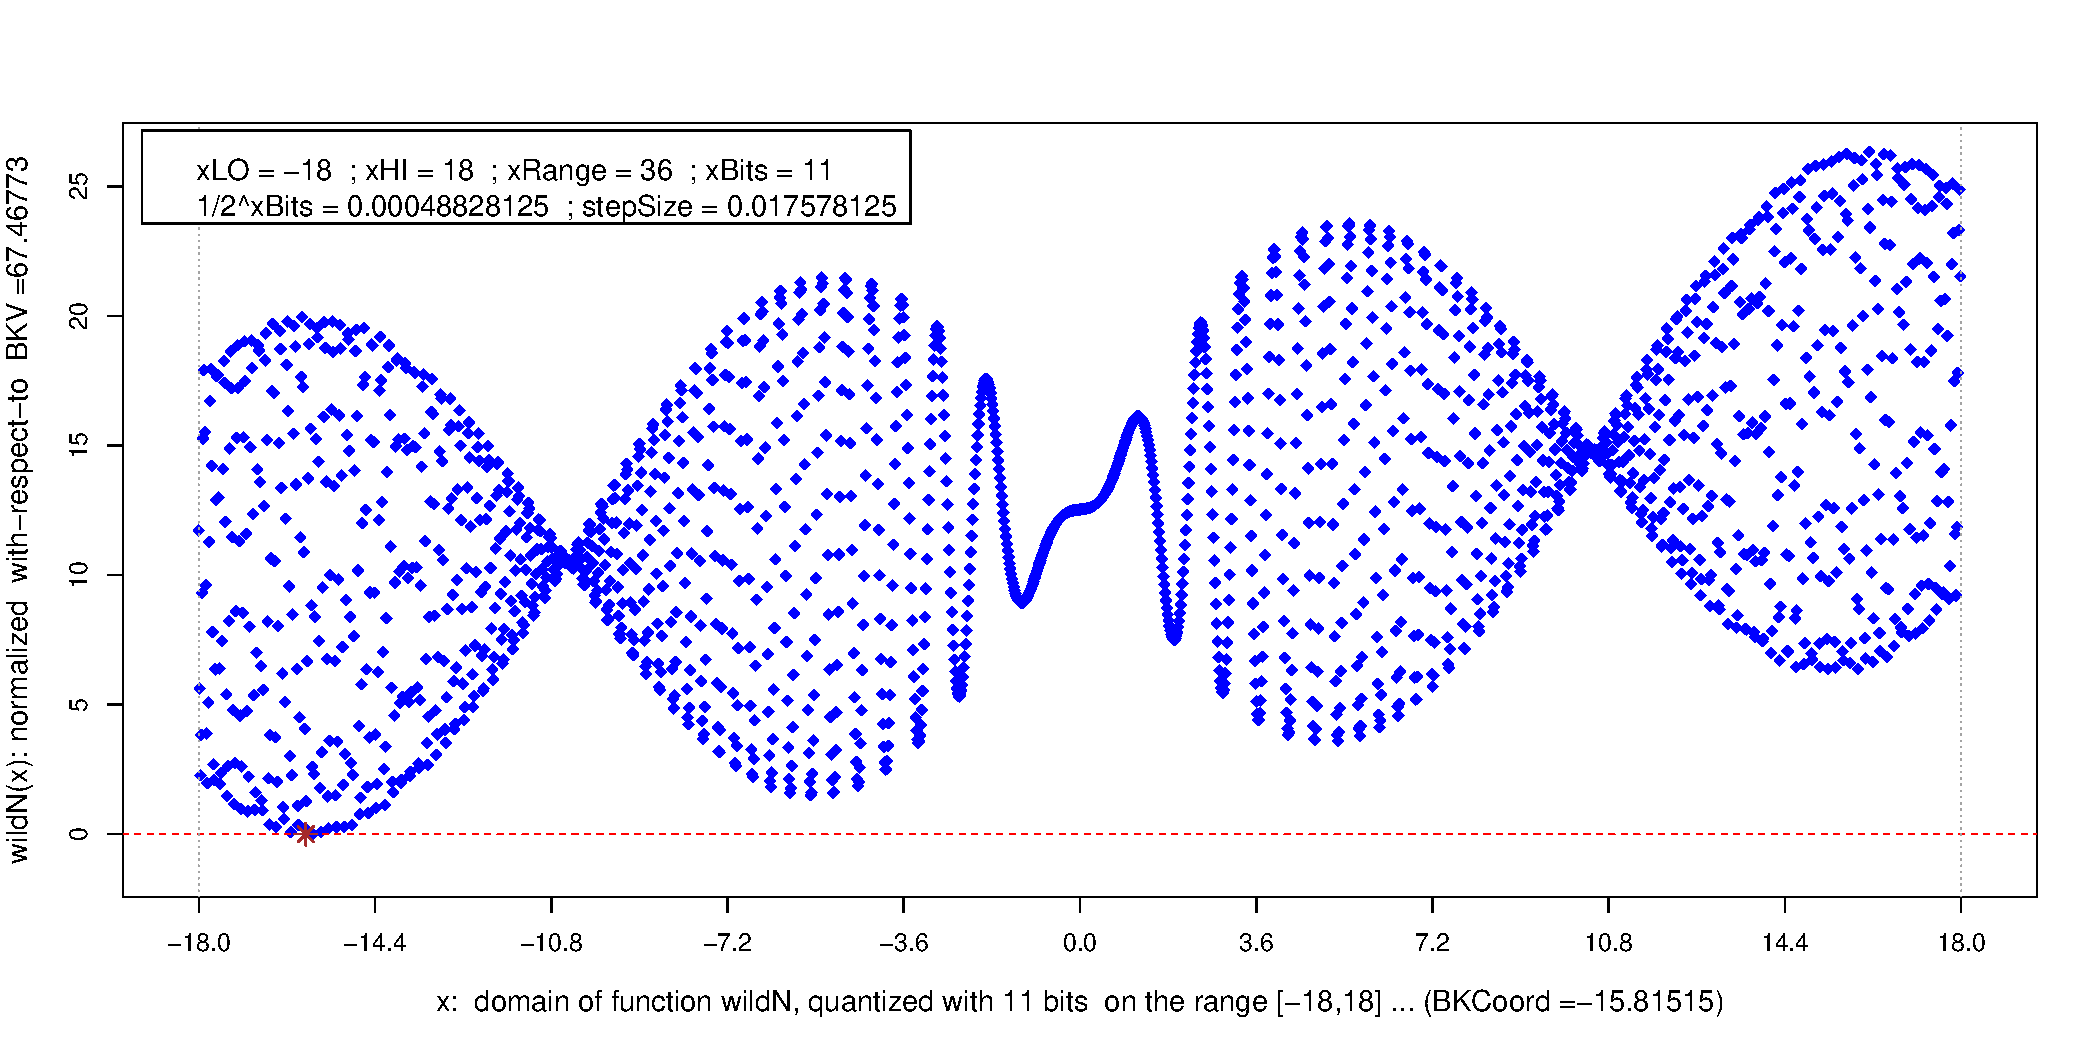
\includegraphics[width=1\linewidth]{fg_OF_wildN_quant_exh.pdf}
    \caption{Function wildN Normalized With Respect To BKV}
   \end{figure}
   
   \begin{figure}
   \centering
   \begin{subfigure}{.5\textwidth}
       \centering
       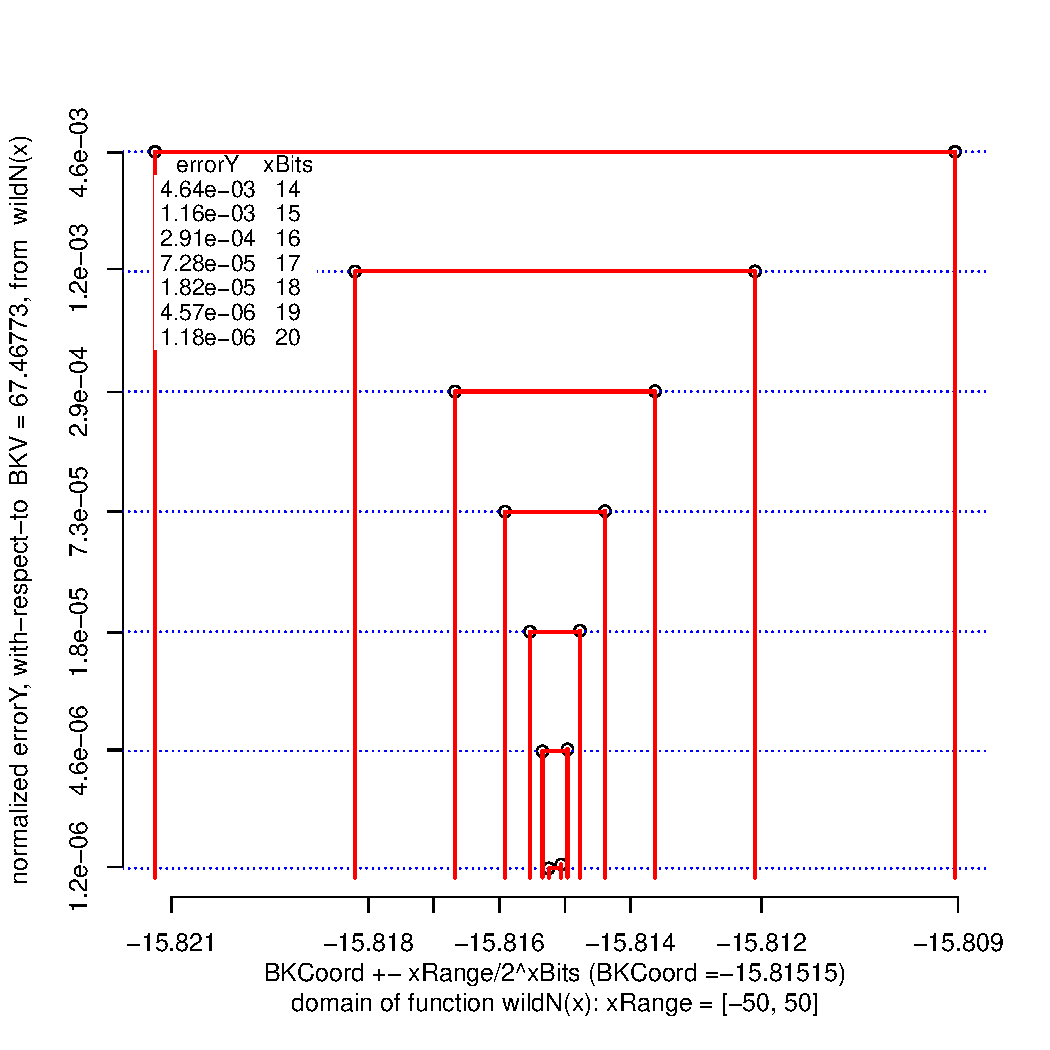
\includegraphics[width=1\linewidth]{fg_OF_wildN_quant_box.pdf}
       \caption{Normalized Error of Function wildN }
   \end{subfigure}%
   \begin{subfigure}{.5\textwidth}
      \centering
      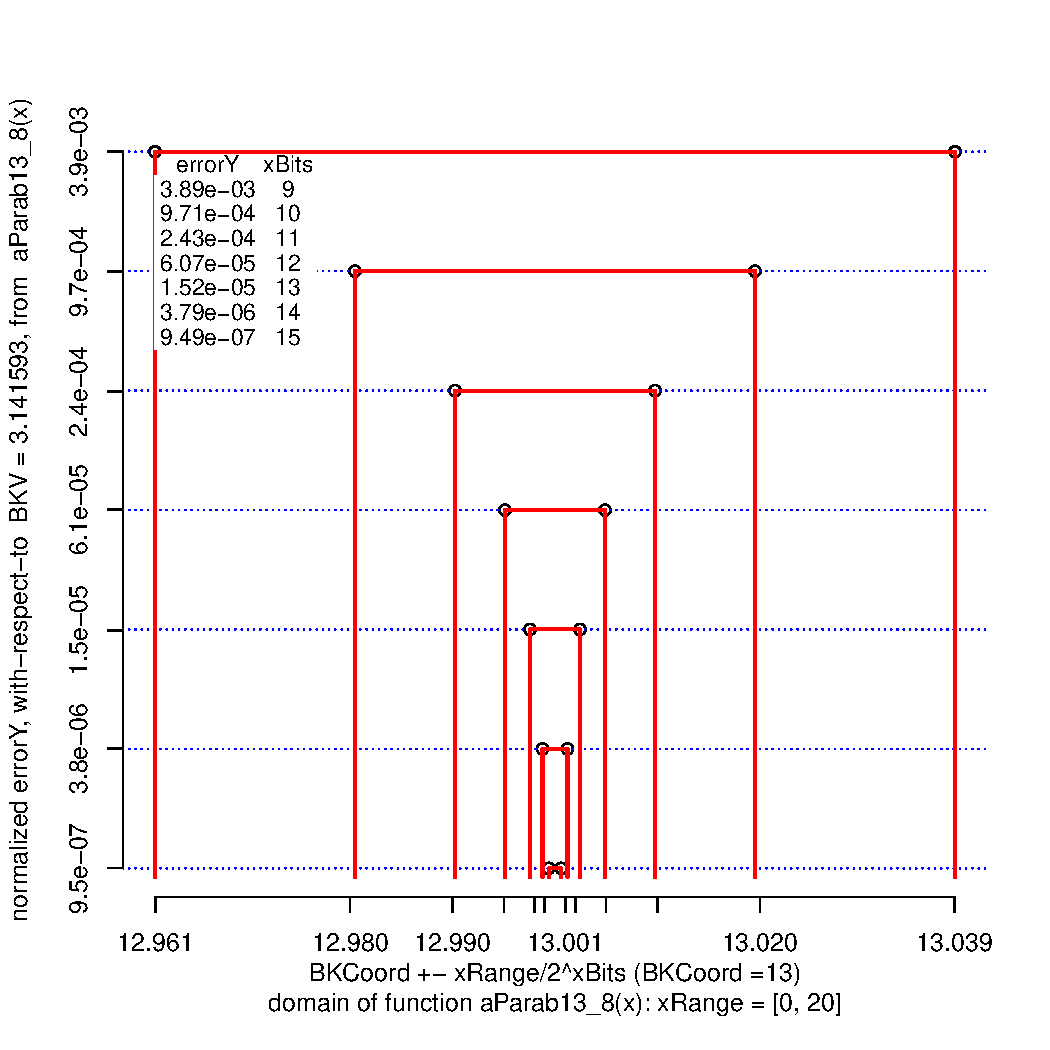
\includegraphics[width=1\linewidth]{fg_OF_aParab13_8_quant_box.pdf}
      \caption{Normalized Error of Function aParab13\_8}
   \end{subfigure}
   \caption{Errors of the Two Objective Functions}
   \end{figure}

\pagebreak

\begin{verbatim} 
<hash> containing 3 key-value pair(s).
  wildN.BKV : 67.46773
  wildN.isValueOnly : FALSE
  wildN.tolY : 0.005

seedInit   = 2657 
solver     = DEoptim 
OFname     = wildN 
nPar       = 1 
nDim       = 1 
lowerBnd   = -50 
upperBnd   = 50 
popSize    = 64 
iterLmt    = 200 
iterCnt    = 7 
tolY       = 5.000e-03 
errorY     = 4.983e-03 
isCensored = FALSE 
BKV        = 67.46773 
BKVcomb    = 67.46773 
BKcoord    = -15.81515 
valueBest  = 0 
coordBest  = -15.35568 

***** summary of DEoptim object ***** 
best member   :  -15.3556778890043 
best value    :  0 
after         :  7 generations 
fn evaluated  :  16 times 
*************************************

 \end{verbatim}
   
   
\end{document}